% Compile with XeLaTeX or LuaLaTeX
\documentclass[10pt]{article}  % Spivak uses ~10pt

% -----------------------------
% Fonts
% -----------------------------
\usepackage{fontspec}
\setmainfont{TeX Gyre Pagella}
\usepackage{unicode-math}
\setmathfont{Libertinus Math}

% -----------------------------
% Page layout
% -----------------------------
\usepackage[margin=2.5cm]{geometry}
\usepackage[parfill]{parskip}

% -----------------------------
% Theorems and QED
% -----------------------------
\usepackage{amsthm}
\usepackage{tcolorbox}
\tcbuselibrary{breakable}

% QED symbol like Spivak (tall gray rectangle)
\renewcommand{\qedsymbol}{\textcolor{black}{\rule{1ex}{2.2ex}}}

\newtheorem{theorem}{Theorem}
\newtheorem{axiom}{Axiom}
\newtheorem{definition}{Definition}

% -----------------------------
% Misc packages
% -----------------------------
\usepackage{graphicx, subfig}
\usepackage{booktabs, array}
\usepackage{paralist, verbatim}
\usepackage{xcolor, pagecolor}
\usepackage{fancyhdr}
\pagestyle{fancy}
\renewcommand{\headrulewidth}{0pt}
\lhead{}\chead{}\rhead{}
\lfoot{}\cfoot{\thepage}\rfoot{}
\usepackage{sectsty}
\allsectionsfont{\sffamily\mdseries\upshape}
\usepackage[nottoc,notlof,notlot]{tocbibind}
\usepackage[titles,subfigure]{tocloft}
\renewcommand{\cftsecfont}{\rmfamily\mdseries\upshape}
\renewcommand{\cftsecpagefont}{\rmfamily\mdseries\upshape}
\usepackage{changepage, comment}
% Define a light gray
\definecolor{lightgraypaper}{RGB}{240,240,240}
% Set the page background
\pagecolor{lightgraypaper}
\color{black} % keep text black

\title{Calculus by Elliott Mendelson}
\author{Noah Lewis}
\begin{document}
\maketitle

\tableofcontents

% ===============================
% 30-Week Calc 1 & Calc 2 Review Schedule
% ===============================

\section{Functions}
\subsection{Some Standard Mappings of the Plane}

\begin{tcolorbox}[title=Problem 1, breakable]
    Let $F$ be a mapping of the plane into itself.
    We define a \textbf{fixed point} for $F$ to be a 
        point $P$ such that $F(P) = P$. \\

    Describe the fixed points of the following mappings.

    (a) The identity.

    (b) Reflection through a given point $O$.

    (c) Reflection through a line.

    (d) A rotation not equal to the identity, with respect to a given point $O$.

    (e) A translation not equal to the identity.

    (f) Dilation by a number $r > 0$, relative to a given point $O$.
\end{tcolorbox}

\textbf{Solution (a):}

All points in the plane are fixed points.

\textbf{Solution (b):}

The point $O$ is a fixed point.

\textbf{Solution (c):}

All points on the line are fixed points.

\textbf{Solution (d):}

The point $O$ is a fixed point.

\textbf{Solution (e):}

There are no fixed points on the plane.

\textbf{Solution (f):}

If $r = 1$, then all points are fixed points.  
If $r \neq 1$, then only $O$ is a fixed point.

\subsection{Isometries}

\begin{tcolorbox}[title=Problem 2, breakable]
    For which values of $r$ is dilation by $r$ an isometry?
\end{tcolorbox}

When $r = 1$ or $r = -1$.

\begin{tcolorbox}[title=Problem 4, breakable]
    Let $L, K$ be two parallel lines, and let $F$ be an isometry.
    Prove that $F(L)$ and $F(K)$ are parallel.
\end{tcolorbox}

\begin{proof}
    If $L = K$ then trivially $F(L)$ and $F(K)$ are parallel as they are equal
        since $F$ is an isometry.

    Suppose $L \not = K$.
    For contradiction, suppose $F(L)$ and $F(K)$ are not parallel.
    Then there is a point where $F(L)$ and $F(K)$ intersect.
    Since $F$ is an isometry, this would imply that $L$ and $K$ also intersect,
        contradicting the fact that $L$ and $K$ are distinct parallel lines.
\end{proof}

\begin{tcolorbox}[title=Problem 5, breakable]
    Let $K, L$ be perpendicular lines, and let $F$ be an isometry.
    Prove that $F(K)$ and $F(L)$ are perpendicular. [Hint: Use the 
    corollary of the Pythagoras theorem.]
\end{tcolorbox}

\begin{proof}
    Let $I$ be the intersection of the lines $K$ and $L$.
    Let $P$ and $Q$ be two points lying on the line $L$ which are equal distances from $I$.
    Let $O$ be a point on $K$ such that $O \ne I$.
    By the corollary to the Pythagorean Theorem, $d(P, O) = d(Q, O)$.
    Now $F(P), F(Q)$ determine a line and $F(O), F(I)$ determine a line (corollary in the text).
    Then, since $F$ is an isometry, $d(F(P), F(O)) = d(F(Q), F(O))$.
    It then follows that the line formed by $F(O), F(I)$ is the perpendicular bisector of $F(P), F(Q)$.
\end{proof}

\begin{tcolorbox}[title=Problem 6, breakable]
    Visualize $3$-dimensional space. We also have the notion of distance in
    space, satisfying the same basic properties as in a plane. We can therefore
    define an isometry of $3$-space in the same way that we defined an isometry
    of the plane. It is a mapping of 3-space into itself which is distance
    preserving. Are Theorems $1$ and $2$ valid in $3$-space? How would you
    formulate Theorem $3$? (Consider the plane in which the three points
    lie.) Now formulate a theorem in 3-space about an isometry being the
    identity provided that it leaves enough points fixed. Describe a proof
    for such a theorem, similar to the proof of Theorem 3. Make a list of
    what you need to assume to make such a proof go through. Write all of
    this up as if you were writing a book. Aside from learning mathematical
    substance, you will also learn how to think more clearly, and how to
    write mathematics in the process
\end{tcolorbox}

\begin{theorem}
    Let $F$ be an isometry. Let $P$, $Q$, $M$, $S$ be four distinct points which 
    do not lie on the same plane. Assume that $P, Q, M, S$ are fixed points of $F$;
    that is
        \[F(P) = P, F(Q) = Q, F(M) = M, F(S) = S\]
    Then $F$ is the identity.
\end{theorem}

The proof could be layed out as follows.
\begin{enumerate}
    \item First take the plane formed by $P, Q, M$ and by Theorem $3$ all points on that 
          plane are fixed points.
    \item Then note that point $S$ does not lie on this plane.
    \item Then since $F$ is an isometry the $d(P, S) = d(F(P), F(S))$,
          $d(Q, S) = d(F(Q), F(S))$, and $d(M, S) = d(F(M), F(S))$.
    \item Determine that $F(S) = S$, and hence that all points of space are fixed; therefore $F$ is the identity.
\end{enumerate}

\subsection{Composition of Isometries}

\begin{tcolorbox}[title=Problem 1, breakable]
    Let $F$ be a reflection through a line $L$. What is the smallest positive 
    integer $n$ such that $F^n = I$.
\end{tcolorbox}

\text{Solution:}

$n = 2$.

\begin{tcolorbox}[title=Problem 4, breakable]
    Give an example of two isometries $F_1$, $F_2$ such that 
    \[F_1 \circ F_2 \ne F_2 \circ F_1\]
\end{tcolorbox}

\text{Solution:}

Let $G_x = $ rotation by $x$\textdegree about the origin.
Let $T_1 = $ translation of $1$ to the right.
Then let $F_1 = G_{45}$ and $F_2 = T_1$.  
These two isometries do not commute
\[
F_1 \circ F_2 \ne F_2 \circ F_1.
\]

\subsection{Inverse of Isometries}

\begin{tcolorbox}[title=Problem 1, breakable]
    (a) Let $F$ be an isometry which has an inverse $F^{-1}$.
    Let $S$ be a circle of radius $r$, and center $P$.
    Show that the image of $S$ under $F$ is a circle.
    [Hint: Let $S'$ be the circle of center $F(P)$ and radius $r$.
    Show that $F(S)$ is contained in $S'$ and that every point of $S'$
    is the image under $F$ of a point in $S$.]

    (b) Let $F$ be an isometry which has an inverse $F^{-1}$.
    Let $D$ be a disc of radius $r$ and center $P$.
    Show that the image of $D$ under $F$ is a disc.
\end{tcolorbox}

\begin{proof}
    Let $S'$ be the circle of center $F(P)$ and radius $r$.
    We need to show that $F(S) \subseteq S'$ and $S' \subseteq F(S)$.

    We first show $F(S) \subseteq S'$. Let $T$ be a point such that $d(P, T) = r$.
    Since $F$ is an isometry $d(F(P), F(T)) = r$.
    Since $T$ was arbitrary all points $T$ such that $d(P, T) = r$
        are contained within the circle centered at 
        $F(P)$ with radius $r$ which is exactly $S'$.

    We now show $S' \subseteq F(S)$. 
    Let $T$ be a point at distance $r$ from the center $F(P)$ of the circle $S'$.
    Now let $Y = F^{-1}(T)$. It follows that $F(Y) = T$.
    We know that  $d(F(Y), F(P)) = r$.
    Since $F$ is an isometry $d(Y, P) = r$.
\end{proof}

\begin{proof}
    Let $D'$ be the disc of center $F(P)$ and radius $r$.
    We need to show that $F(D) \subseteq D'$ and $D' \subseteq F(D)$.

    We first show $F(D) \subseteq D'$. Let $T$ be a point such that $d(P, T) \le r$.
    Since $F$ is an isometry, $d(F(P), F(T)) \le r$.
    Since $T$ was arbitrary, all points $T$ with $d(P, T) \le r$
        are contained within the disc centered at $F(P)$ with radius $r$, which is exactly $D'$.

    We now show $D' \subseteq F(D)$. 
    Let $T$ be a point at distance $\le r$ from the center $F(P)$ of the disc $D'$.
    Now let $Y = F^{-1}(T)$. It follows that $F(Y) = T$.
    We know that $d(F(Y), F(P)) \le r$.
    Since $F$ is an isometry, $d(Y, P) \le r$.
\end{proof}

\begin{tcolorbox}[title=Problem 2, breakable]
    Let $P, Q, P', Q'$ be points such that 
    \[d(P, Q) = d(P', Q')\]
    Prove that there exists an isometry $F$ such that $F(P) = P'$
    and $F(Q) = Q'$.
    You may assume the statements we have assumed in this section.
\end{tcolorbox}

\begin{proof}
    First, perform a rotation $G$ of $Q$ about $P$ such that the line formed by $P$ and $Q$ is parallel to 
    the line formed by $P'$ and $Q'$.
    
    Next, let $T$ be the translation along the ray from $Q$ to $Q'$ of length $d(Q, Q')$.
    Applying $T$ moves $Q$ exactly to $Q'$. 
    Since the line through $P$ and $Q$ is parallel to the line through $P'$ and $Q'$, the same translation
    moves $P$ to $P'$.
    
    Since rotations and translations are isometries, the composition $T \circ G$ is an isometry.
\end{proof}

\begin{tcolorbox}[title=Problem 3, breakable]
    Let $F, G, H$ be isomemetries and assume that $F$ has an inverse.
    If \[F \circ G = F \circ H\]
    prove that $G = H$ (\textbf{cancellation law} for isomemetries).
\end{tcolorbox}

\begin{proof}
    Applying $F^{-1}$ to both sides yields 
    \begin{align*}
        &F^{-1} \circ (F \circ G) = F^{-1} \circ (F \circ H) \\
        \iff& (F^{-1} \circ F) \circ G = (F^{-1} \circ F) \circ H \\
        \iff& I \circ G = I \circ H \\
        \iff& G = H
    \end{align*}
\end{proof}

\begin{tcolorbox}[title=Problem 4, breakable]
    (a) Let $F$ be an isometry such that $F^2 = I$ and $F^3 = I$.
        Prove that $F = I$. \\

    (b) Let $F$ be an isometry such that $F^4 = I$ and $F^7 = I$.
        Prove that $F = I$. \\

    (c) Let $F$ be an isometry such that $F^5 = I$ and $F^8 = I$.
        Prove that $F = I$.
\end{tcolorbox}

\begin{proof}
    Since $F^2 = I$ it follows that $F^3 = F \circ I$.
    Then $F = F \circ I  = F^3 = I$.
\end{proof}

\begin{proof}
    Since $F^4 = I$ it follows that $I = F^{-4} \circ I = F^{-4}$.
    Also since $F^4 = I$ it follows that $F = F^{-3} \circ I = F^{-3}$.
    Then $F = F^{-3} = F^{7} \circ F^{-4} = I \circ I = I$.
\end{proof}

\begin{proof}
    Since $F^5 = I$ it follows that $F = F^{-4} \circ I = F^{-4}$.
    Also, since $F^8 = I$ it follows that $F^3 = F^{-5} \circ I = F^{-5}$.
    Finally, since $F^8 = I$ it follows that $I = F^{-8} \circ I = F^{-8}$.
    Then
    \[F = F^{-4} \circ I  = F^{-4} \circ F^{-8} = F^{-12} = F^{-5} \circ F^{-8} = F^3 \circ F^{-8}  = F^3 \circ F^{-4} \circ F^{-4} = F^3 \circ F \circ F = F^5 = I \]
\end{proof}

\begin{tcolorbox}[title=Problem 5, breakable]
    Write out the proof of the corollary of Theorem $3$. (Consider $F^{-1} \circ G$.)
\end{tcolorbox}

\begin{figure}[h]
    \centering
    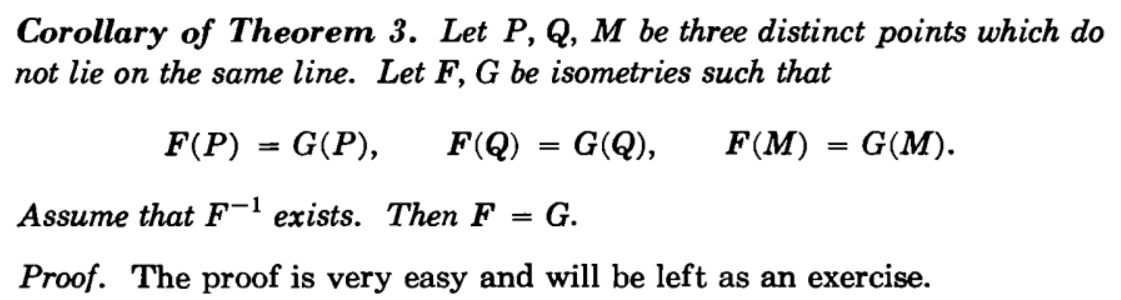
\includegraphics[width=0.6\textwidth]{images/coral.png}
\end{figure}

\begin{proof}
    Since $F(P) = G(P)$, $F(Q) = G(Q)$, and $F(M) = G(M)$
        it follows that $P = (F^{-1} \circ G)(P)$, $Q = (F^{-1} \circ G)(Q)$, and $M = (F^{-1} \circ G)(M)$.
    Now this is three fixed points so $F^{-1} \circ G$ is the identity mapping.
    Since $F^{-1} \circ G = I$ it follows that $G$ is the inverse of $F^{-1}$ which is $F$.
\end{proof}

\begin{tcolorbox}[title=Problem 6, breakable]
    Let $F \circ G \circ H$ be the composite of three isometries.
    Assume that $F^{-1}$, $G^{-1}$, $H^{-1}$ exist.
    Prove that $(F \circ G \circ H)^{-1}$ exists, and express this 
    inverse in terms of the inverses for $F, G, H$.
\end{tcolorbox}

\begin{proof}
    Let $P$ be an arbitrary point in the plane such that $(F \circ G \circ H)(P) = X$.
    Then 
    \begin{align*}
        &(F \circ G \circ H)(P) = X \\
        \iff& (H^{-1} \circ (F \circ G \circ H))(P) = H^{-1}(X) \\
        \iff& ((G^{-1} \circ H^{-1}) \circ (F \circ G \circ H))(P) = (G^{-1} \circ H^{-1})(X) \\
        \iff& ((F^{-1} \circ G^{-1} \circ H^{-1}) \circ (F \circ G \circ H))(P) = (F^{-1} \circ G^{-1} \circ H^{-1})(X) \\
        \iff& ((F \circ G \circ H)^{-1} \circ (F \circ G \circ H))(P) = (F^{-1} \circ G^{-1} \circ H^{-1})(X) \\
        \iff& I(P) = (F^{-1} \circ G^{-1} \circ H^{-1})(X) \\
        \iff& P = (F^{-1} \circ G^{-1} \circ H^{-1})(X)
    \end{align*}
    Therefore, $(F \circ G \circ H)^{-1} = H^{-1} \circ G^{-1} \circ F^{-1}$.
\end{proof}

\begin{tcolorbox}[title=Problem 7, breakable]
    Let $F$ be an isometry such that $F^7 = I$.
    Express $F^{-1}$ as a positive power $F$.
\end{tcolorbox}

\begin{proof}
Since $F^7 = I$, we have
\[
F^{-1} = I \circ F^{-1} = F^7 \circ F^{-1} = F^6.
\]
\end{proof}

\begin{tcolorbox}[title=Problem 8, breakable]
    Let $n$ be a positive integer and let $F$ be an isometry such that $F^n = I$.
    Express $F^{-1}$ as a positive power of $F$.
\end{tcolorbox}

\begin{proof}
    Since $F^n = I$, we have
\[
F^{-1} = I \circ I  \circ F^{-1} = F^n \circ F^n \circ F^{-1} = F^{2n - 1}.
\]
    Since $n \ge 1$ it follows that $2n \ge 2$ so $2n > 1$ and $2n - 1 > 0$.
\end{proof}

\begin{tcolorbox}[title=Problem 9, breakable]
    Consider the corners of a square centered at the origin.
    For convenience of notation, number these corners $1, 2, 3, 4$ as in Fig. $6-26$.

    Write the image of each one of these corners under the isometries.
    $H, V, H \circ V, V \circ H$. Just to show you an easy notation to 
    do this, we write down the images of these corners under rotation by 
    $90$\textdegree in the following form:

    \[
    \begin{bmatrix}
    1 & 2 & 3 & 4 \\
    2 & 3 & 4 & 1
    \end{bmatrix}
    \]

    This notation means that if $G$ is a rotation by $90$\textdegree,
    then $G(1) = 2$, $G(2) = 3$, $G(3) = 4$, and $G(4) = 1$.

    $H, V$ are the reflections along the horizontal line 
        and vertical line respectively.
\end{tcolorbox}

\begin{figure}[h]
    \centering
    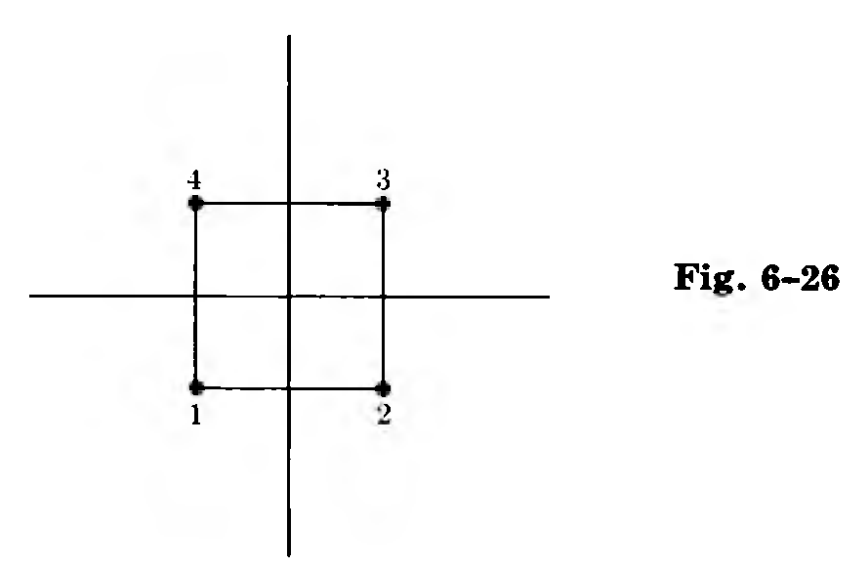
\includegraphics[width=0.6\textwidth]{images/square.png}
\end{figure}

\textbf{Solution:}

Image under $H$.
\[
\begin{bmatrix}
1 & 2 & 3 & 4 \\
4 & 3 & 2 & 1
\end{bmatrix}
\]
Image under $V$.
\[
\begin{bmatrix}
1 & 2 & 3 & 4 \\
2 & 1 & 4 & 3
\end{bmatrix}
\]
Image under $H \circ V$.
\[
\begin{bmatrix}
1 & 2 & 3 & 4 \\
3 & 4 & 1 & 2
\end{bmatrix}
\]
Image under $V \circ H$.
\[
\begin{bmatrix}
1 & 2 & 3 & 4 \\
3 & 4 & 1 & 2
\end{bmatrix}
\]

\begin{tcolorbox}[title=Problem 10, breakable]
    Let $G$ be a rotation by $90$\textdegree so that $G^4 = I$.
    Express $H \circ G \circ H$ as a power of $G$.
    For what positive integer $n$ do we have 
    \[H \circ G = G^n \circ H\]
    Write down the images of the corner of the square as in 
    the preceeding exercize, under the maps 
    $I, G, G^2, G^3, H, H \circ G, H \circ G^2, H \circ G^3, G \circ H, G^2 \circ H, G^3 \circ H$.
\end{tcolorbox}

\textbf{Solution:}

\[H \circ G \circ H = G^3\]
The following equation holds when $n = 3$.
\[H \circ G = G^n \circ H\]
% Identity
Image under $I$.
\[
\begin{bmatrix}
1 & 2 & 3 & 4 \\
1 & 2 & 3 & 4
\end{bmatrix}
\]

% Rotation by 90°
Image under $G$.
\[
\begin{bmatrix}
1 & 2 & 3 & 4 \\
2 & 3 & 4 & 1
\end{bmatrix}
\]

% Rotation by 180°
Image under $G^2$.
\[
\begin{bmatrix}
1 & 2 & 3 & 4 \\
3 & 4 & 1 & 2
\end{bmatrix}
\]

% Rotation by 270°
Image under $G^3$.
\[
\begin{bmatrix}
1 & 2 & 3 & 4 \\
4 & 1 & 2 & 3
\end{bmatrix}
\]

% Reflection H (horizontal)
Image under $H$.
\[
\begin{bmatrix}
1 & 2 & 3 & 4 \\
4 & 3 & 2 & 1
\end{bmatrix}
\]

% H followed by G
Image under $H \circ G$.
\[
\begin{bmatrix}
1 & 2 & 3 & 4 \\
1 & 4 & 3 & 2
\end{bmatrix}
\]

% H followed by G^2
Image under $H \circ G^2$.
\[
\begin{bmatrix}
1 & 2 & 3 & 4 \\
3 & 2 & 1 & 4
\end{bmatrix}
\]

% H followed by G^3
Image under $H \circ G^3$.
\[
\begin{bmatrix}
1 & 2 & 3 & 4 \\
2 & 1 & 4 & 3
\end{bmatrix}
\]

% G followed by H
Image under $G \circ H$.
\[
\begin{bmatrix}
1 & 2 & 3 & 4 \\
3 & 4 & 1 & 2
\end{bmatrix}
\]

% G^2 followed by H
Image under $G^2 \circ H$.
\[
\begin{bmatrix}
1 & 2 & 3 & 4 \\
2 & 1 & 4 & 3
\end{bmatrix}
\]

% G^3 followed by H
Image under $G^3 \circ H$.
\[
\begin{bmatrix}
1 & 2 & 3 & 4 \\
4 & 3 & 2 & 1
\end{bmatrix}
\]

\begin{tcolorbox}[title=Problem 13, breakable]
    Consider a triangle  whose three sides have equal length
    and whose three angles have the same measure, $60$\textdegree,
    as in Fig. $6-27$.

    The vertices of the triangle are numbered $1, 2, 3$.
    Let $G$ be a rotation by $120$\textdegree and let $V$,
    as usual, be reflection through the vertical axis.
    
    (a) Give the effect of the six isometries $I, G, G^2, V, VG, VG^2$
    on the vertices, using the same notation as exercize $9$.

    (b) Make up the multiplication table for these six isometries.
\end{tcolorbox}

\begin{figure}[h]
    \centering
    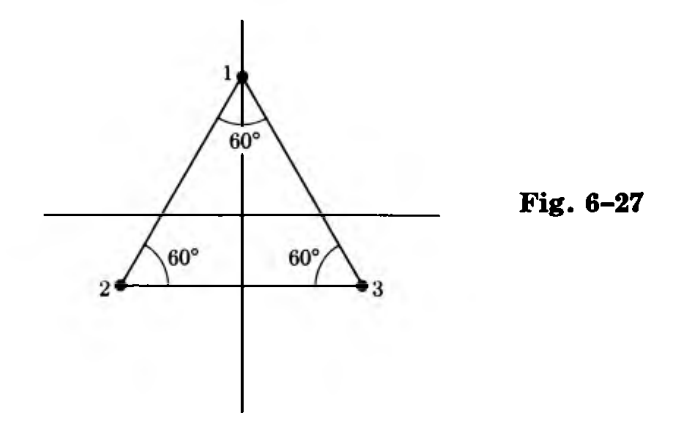
\includegraphics[width=0.6\textwidth]{images/triangle.png}
\end{figure}

\textbf{Solution:}

% Identity
Image under $I$.
\[
\begin{bmatrix}
1 & 2 & 3 \\
1 & 2 & 3
\end{bmatrix}
\]

% Rotation by 120°
Image under $G$.
\[
\begin{bmatrix}
1 & 2 & 3 \\
2 & 3 & 1 
\end{bmatrix}
\]

% Rotation by 240°
Image under $G^2$.
\[
\begin{bmatrix}
1 & 2 & 3 \\
3 & 1 & 2
\end{bmatrix}
\]

% Reflection by vertical
Image under $V$.
\[
\begin{bmatrix}
1 & 2 & 3  \\
1 & 3 & 2
\end{bmatrix}
\]

% Reflection by vertical and rotation by 120°
Image under $VG$.
\[
\begin{bmatrix}
1 & 2 & 3  \\
3 & 2 & 1
\end{bmatrix}
\]

% Reflection by vertical and rotation by 240°
Image under $VG^2$.
\[
\begin{bmatrix}
1 & 2 & 3  \\
2 & 1 & 3
\end{bmatrix}
\]

\[
\begin{array}{c|cccccc}
\circ & I & G & G^2 & V & VG & VG^2 \\ \hline
I & I & G & G^2 & V & VG & VG^2 \\
G & G & G^2 & I & VG^2 & V & VG \\
G^2 & G^2 & I & G & VG & VG^2 & V \\
V & V & VG & VG^2 & I & G^2 & G \\
VG & VG & VG^2 & V & G & I & G^2 \\
VG^2 & VG^2 & V & VG & G^2 & G & I
\end{array}
\]

\subsection{Characterization of Isometries}

\begin{tcolorbox}[title=Problem 1, breakable]
    Prove that every isometry has an inverse.
\end{tcolorbox}

\begin{proof}
    Let $F$ be an arbitrary isometry.
    There are four cases depending on the number of 
        fixed points under $F$.

    (\textbf{$\ge3$ fixed points}) By Theorem $3$, $F = I$
        which clearly has an inverse: $F^{-1} = I$.

    (\textbf{$2$ fixed points}) 
        Let $P$ and $Q$ be the two fixed points under $F$.
        By Theorem $4$, either $F$ is the identity, or $F$ is a reflection
        through the line $L_{PQ}$ passing through $P$ and $Q$.
        In the identity case, $F^{-1} = I$.
        If $F$ is a reflection, the inverse is also $F$: $F^{-1} = F$.

    (\textbf{$1$ fixed point}) 
        Let $P$ be the single fixed point under $F$.
        By Theorem $5$, either $F$ is a rotation about $P$, or 
        $F$ is a rotation composed with a reflection through a line through $P$.
        In the rotation case, $F^{-1}$ is the rotation by the opposite angle about $P$.
        In the rotation-reflection case, $F^{-1}$ is the reflection composed with the rotation by the opposite angle.

    (\textbf{no fixed points})
        By Theorem $6$, either $F$ is a translation,
            a composite of a translation and a rotation,
            or a composite of a translation, a rotation, and a reflection through a line.
        In the translation case, $F^{-1}$ is the translation by the opposite vector.
        In the translation-rotation case, $F^{-1}$ is the rotation by the opposite angle followed by translation by the opposite vector.
        In the translation-rotation-reflection case, $F^{-1}$ is the reflection followed by rotation by the opposite angle and translation by the opposite vector.

    Since these cases are exhaustive, every isometry has an inverse.
\end{proof}

\begin{tcolorbox}[title=Problem 2, breakable]
    If $P$ is a fixed point for an isometry $F$,
        prove that $P$ is also a fixed point 
        for $F^{-1}$.
\end{tcolorbox}

\begin{proof}
    Since $P$ is a fixed point under $F$ is follows that $F(P) = P$.
    By Problem $1$ we know that $F^{-1}$ exists.
    Applying $F^{-1}$ to both sides yields $P = F^{-1}(P)$.
    Therefore, $P$ is a fixed point of $F^{-1}$.
\end{proof}

\subsection{Congruences}

\newpage
\begin{tcolorbox}[title=Problem 1, breakable]
    Prove that two discs of the same radius are congruent.
\end{tcolorbox}

\begin{proof}
    Let the first disc be $D(r, O)$, of radius $r$, centered at $O$, and let
    the other disc be $C(r, O')$, centered at $O'$. Let $T$ be the translation which
    maps $O$ on $O'$. We know that $T$ preserves distances. Hence if $P$ is at distance
    $\le r$ from $O$, then $T(P)$ is at distance $\le r$ from $T(O) = O'$. Hence the image of the
    disc $D(r, O)$ is contained in the circle $D(r, O')$. We must still show that every
    point on $D(r, O')$ is the image of a point on $D(r, O)$ under T. Let Q be a point
    at distance $\le r$ from $O'$. Note that the point
    \[P = T^{-1}(Q)\]
    is at distance $\le r$ from $O$, and that $T(P) = T(T^{-1}(Q)) = Q$.
\end{proof}

\begin{tcolorbox}[title=Problem 2, breakable]
    Let $S, S', S''$ be sets in the plane.
    Prove that if $S$ is congruent to $S'$,
        and $S'$ is congruent to $S''$,
        then $S$ is congruent to $S''$.
    Prove that if $S$ is congruent to $S'$,
        then $S'$ is congruent to $S$.
\end{tcolorbox}

\begin{proof}
    Suppose that $S$ is congruent to $S'$ and $S'$ is congruent to $S''$.
    Let $T$ be the isometry such that $T(S) = S'$.
    Let $F$ be the isometry such that $F(S') = S''$.
    Then $(F \circ T)(S) = F(T(S)) = F(S') = S''$.
    Note that a composition of isometries is an isometry.
    Thus $F \circ T$ is an isometry mapping $S$ to $S''$ 
        so $S$ is congruent to $S''$.
\end{proof}

\begin{proof}
    Suppose that $S$ is congruent to $S'$.
    Let $F$ be the isometry such that $F(S) = S'$.
    Since $F$ is an isometry it has an inverse $F^{-1}$.
    Then applying this to both sides yields $S = F^{-1}(S')$.
    Thus $S'$ is congruent to $S$.
\end{proof}

\begin{tcolorbox}[title=Problem 3, breakable]
    Prove that two squares whose sides have the 
        same length are congruent.
\end{tcolorbox}

\begin{proof}
    Let $S$ and $S'$ be two squares whose sides have the same length.
    Let $A, B, C, D$ be the vertices of $S$ in cyclic order.
    Let $O$ be the intersection of the diagonals $AC$ and $BD$.
    Since the diagonals of a square are equal in length and bisect each other
        at right angles, their intersection $O$ is equidistant from all vertices.
    Thus $O$ is the center of $S$.

    Similarly, let $A', B', C', D'$ be the vertices of $S'$ in cyclic order,
    and let $O'$ be the intersection of its diagonals (the center of $S'$).

    Let $T$ be the translation mapping $O$ to $O'$.
    Let $G$ be the rotation with respect to $O'$
        of $S'$ such that $(G \circ T)(A) = A'$.
    Because $G$ is a rotation about the center $O'$, it must also send 
        the point on the opposite end of that diagonal, namely $(G\circ T)(C)$, to $C'$, 
        and $(G\circ T)(D)$ to $D'$.
    If $(G \circ T)(B) \neq B'$, then perform  
        a reflection $R$ across the line connecting $(G \circ T)(A)$ and $(G \circ T)(C)$.
    Otherwise, let $R = I$ such that $I$ is the identity mapping.
    Let $F = R \circ G \circ T$.

    Thus $F(A) = A', F(B) = B', F(C) = C', F(D) = D'$, 
        and therefore $F(S) \subseteq S'$.
    Since $F$ is an isometry, it preserves distances and lines, so 
    every point of $S$ maps to points of $S'$ and vice versa, thus $F(S) = S'$.
\end{proof}

\newpage
\begin{tcolorbox}[title=Problem 4, breakable]
    Prove that any two lines are congruent.
\end{tcolorbox}


\begin{proof}
    Let $L$ and $L'$ be two lines. Pick points $P, Q \in L$ and $P', Q' \in L'$.  
    Using Section $6.4$ Problem $2$, since $d(P,Q) = d(P',Q')$, there exists an isometry $F$ such that $F(P) = P'$ and $F(Q) = Q'$.  

    Since $F$ preserves distances and maps two points on $L$ to two points on $L'$, it maps the entire line $L$ onto $L'$.  
    Therefore, the lines $L$ and $L'$ are congruent.
\end{proof}

\begin{tcolorbox}[title=Problem 5, breakable]
    Let $\triangle ABC$ be a triangle whose three angles all have $60$\textdegree.
    Prove that the sides have equal length.
    [Hint: From any vertex draw the perpendicular to the other side,
           and reflect through this perpendicular.]
\end{tcolorbox}

\begin{proof}
    Let $A, B, C$ be the vertices of a triangle whose three angles all have $60$\textdegree.
    Let $L$ be the perpendicular bisector of $\overline{AB}$, intersecting $\overline{AB}$ at its midpoint $O$.
    There are now two right triangles, namely $\triangle AOC$ and $\triangle BOC$,
        with right angles at $O$.
    These triangles share the side $\overline{OC}$.
    Since $L$ is the perpendicular bisector of $\overline{AB}$, we have $d(A, O) = d(B, O)$.
    Then
    \[
        d(A, C)^2 = d(A, O)^2 + d(O, C)^2 = d(B, O)^2 + d(O, C)^2 = d(B, C)^2.
    \]
    It follows that $d(A, C) = d(B, C)$.
    
    Apply similar steps but let $L$ be the perpendicular bisector of $\overline{BC}$,
        thus showing that $d(A, B) = d(A, C)$.

    Thus $d(A, B) = d(A, C) = d(B, C)$.
\end{proof}

\begin{proof}
    Let $A, B, C$ be the vertices of a triangle with all angles $60$\textdegree.
    Consider the perpendicular bisector $L$ of side $\overline{AB}$.
    Reflect the vertex $C$ across $L$ to a point $C'$. 

    Since the triangle has equal angles, this reflection maps the triangle to itself, so $C' = C$. 
    Reflection across the perpendicular bisector preserves distances, so
    \[
        AC = BC.
    \]
    Similarly, reflecting across the perpendicular bisector of $\overline{BC}$ gives
    \[
        AB = AC.
    \]
    Therefore, all three sides are equal:
    \[
        AB = BC = AC.
    \]
\end{proof}

\newpage
\begin{tcolorbox}[title=Problem 6, breakable]
    Prove Theorem $9$.
    At first you are not allowed to use Theorem $10$.
    If you were allowed to use Theorem $10$, how would 
        you deduce Theorem $9$ from it.

    \begin{theorem}
        Let $\triangle PQM$ and $\triangle P'Q'M'$ be right triangles 
            whose right anlges are at $Q$ and $Q'$ respectively.
        Assume that the corresponding legs have the same lengths,
            that is:
        \[d(P, Q) = d(P', Q')\]
        and 
        \[d(Q, M) = d(Q', M')\]
        Then the triangles are congruent.
    \end{theorem}
\end{tcolorbox}

\begin{proof}
    Let $T$ be the translation such that $T(Q) = Q'$.
    Let $G$ be the ration such that $(G \circ T)(P) = P'$.
    Finally, if $(G \circ T)(M) \not = M'$ apply a reflection on the line $\overline{P'Q'}$
    Let $F = G \circ T$.

    Thus, $G(Q) = Q'$, $G(P) = P'$, and $G(M) = M'$.

    Now let $O$ be any point on the segment $\overline{PQ}$.
    It follows that $d(P, Q) = d(F(P), F(Q)) = d(P, O) + d(Q, O) = d(F(P), F(O)) + d(F(Q), F(O))$.
    Then since $d(F(P), F(Q)) = d(F(P), F(O)) + d(F(Q), F(O))$, $F(O)$ lies on the segment $\overline{P'Q'}$.

    Now let $K$ be any point on the segment $\overline{P'Q'}$.
    Since $F$ is an isometry, it has an inverse; let $U = F^{-1}(K)$.
    Then $d(P, Q) = d(F^{-1}(P'), F^{-1}(Q')) = d(P, U) + d(U, Q)$ so $U$ lies on the segment $\overline{PQ}$.
    It follow that  $F(U) = F(F^{-1}(K)) = K$.

    Simlar arguments apply to $\overline{QM}$ and $\overline{PM}$.
    Thus the triangles are congruent.
\end{proof}

\begin{proof}
    Since the legs have the same length, by the Pythagorean Theorem their hypotenuses are of equal length.
    Thus the lengths of the sides of the triangles are equal.
    One can then easily apply Theorem $10$ to show the triangles are congruent.
\end{proof}

\begin{tcolorbox}[title=Problem 7, breakable]
    Let $\triangle PQM$ and $\triangle P'Q'M'$ be triangles 
        having one corresponding angle of the same measure,
        say $\angle PQM$ and $\angle P'Q'M'$ have the same measure,
        and having adjacent sides of the same length, i.e.
        \[d(P, Q) = d(P', Q') \text{ and } d(Q, M) = d(Q', M')\]
        Prove that the triangles are congruent.
\end{tcolorbox}

\begin{proof}
    Let $\triangle PQM$ and $\triangle P'Q'M'$ have a corresponding angle of the same measure, say $\angle PQM = \angle P'Q'M'$, 
    and let the adjacent sides satisfy $d(P,Q) = d(P',Q') \quad \text{and} \quad d(Q,M) = d(Q',M')$.

    Draw the altitude from $Q$ to the side $\overline{PM}$ in $\triangle PQM$, and let $H$ be the foot of this perpendicular.  
    Similarly, draw the altitude from $Q'$ to $\overline{P'M'}$ in $\triangle P'Q'M'$, and let $H'$ be the foot.

    Now consider the right triangles $\triangle QPH$ and $\triangle QMH$ in the first triangle, 
        and $\triangle Q'P'H'$ and $\triangle Q'M'H'$ in the second.  
    By construction and the given distances, 
        the corresponding legs of these right triangles are equal 
        $d(Q,P) = d(Q',P'), \quad d(Q,H) = d(Q',H'), \quad d(Q,M) = d(Q',M'), \quad d(Q,H) = d(Q',H')$

    By Theorem 10, triangles with all three sides equal are congruent, so 
    \[
    \triangle QPH \cong \triangle Q'P'H' \quad \text{and} \quad \triangle QMH \cong \triangle Q'M'H'.
    \]

    Since both pairs of right triangles are congruent, all points $P, Q, M$ correspond to $P', Q', M'$, and therefore
\end{proof}


\begin{tcolorbox}[title=Problem 8, breakable]
    Prove that two rectangles having corresponding sides 
        of equal lengths are congruent.
\end{tcolorbox}

\begin{proof}
    Let $ABCD$ and $A'B'C'D'$ be the corners encountered cyclicly of two rectangles such that 
        $d(A,B) = d(A',B')$ and $d(B,C) = d(B',C')$.

    Let $T$ be the translation such that $T(A) = A'$.
    Let $G$ be the rotation about $A'$ such that $(G \circ T)(C)$ lies on the line through $A'$ and $C'$.
    If necessary, let $R$ be a reflection across the line $\overline{A'C'}$ to match $B$ and $B'$.
    Otherwise, let $R = I$ where $I$ is the identity mapping.
    
    % F should be the composition of those isometries.
    Thus $F = R \circ G \circ T$.

    Draw the diagonal $\overline{AC}$ in both rectangles. 
    This divides each rectangle into two right triangles: 
        $\triangle ABC$ and $\triangle ADC$ in the first rectangle, 
        and $\triangle A'B'C'$ and $\triangle A'D'C'$ in the second.

    Now let $O$ be any point on the segment $\overline{AC}$ of the first rectangle.
    It follows that $d(A,C) = d(A,O) + d(O,C) = d(A',F(O)) + d(F(O),C')$. 
    Then, by the Pythagorean Theorem, $F(O)$ lies on the segment $\overline{A'C'}$.

    Now let $K$ be any point on the segment $\overline{A'C'}$.  
    Since $F$ is an isometry, it has an inverse; let $U = F^{-1}(K)$.  
    Then $d(A,C) = d(F^{-1}(A'), F^{-1}(C')) = d(A,U) + d(U,C)$
        so $U$ lies on the segment $\overline{AC}$.  
    By definition of $U$, $F(U) = F(F^{-1}(K)) = K$.

    Hence the corresponding right triangles along the diagonals are congruent, 
        and therefore the rectangles $ABCD$ and $A'B'C'D'$ are congruent.
\end{proof}

\begin{tcolorbox}[title=Problem 9, breakable]
    Give a definition of the region bounded by a square in terms of line 
        segments. Same thing for a rectangle.
\end{tcolorbox}

\begin{definition}
    Let $S$ be a square with distinct parallel line segments $\overline{AB}$ and $\overline{CD}$.
    We can define the area of $S$ to be all points on all line segments formed by 
        points $X, Y$ where $X$ lies on $\overline{AB}$ and $Y$ lies on $\overline{CD}$.
    The area for a rectangle can be defined in precisely the same way
        with exception to letting $S$ be a rectangle.
\end{definition}

\begin{tcolorbox}[title=Problem 11, breakable]
    Let $\triangle PQM$ and $\triangle P'Q'M'$ be triangles whose corresponding
        angles have the same measures (i.e. the angle with vertex $P$ has the same 
        measure as the angle with vertex at $P'$, and similarly for the angles with
        vertices at $Q, Q'$ and $M, M'$). Assume that $d(P, Q) = d(P', Q')$.
    Prove that the triangles are congruent.
\end{tcolorbox}

\begin{tcolorbox}[title=Problem 12, breakable]
    Let $\triangle PQM$ be a triangle. 
    Let $L_1, L_2, L_3$ be the three lines which bisect 
        the three angles of the triangle, respectively.
    Let $O$ be the point of intersection of $L_1$ and $L_2$.
    Prove that $O$ lies on $L_3$.
    [Hint: From $O$, draw the perpendicular segments to the corresponding sides. 
     Prove that their lengths are equal.]
\end{tcolorbox}
% Week 1: Review domain, range, composition, and inverse functions. Make sure you understand function behavior and graphs.

\section{Limits}
\subsection{Area of a Disc of Radius $r$}

\begin{tcolorbox}[title=Problem 3, breakable]
    (a) Suppose that the sides of a rectangles $S$ have lengths 
        $r$ and $s$. What are the lengths of the sides  of the 
        rectangle $F_{a, b}(S)$, i.e. of the rectangle obtained 
        by the mixed dilation $F_{a, b}$?

    (b) What is the area of $F_{a, b}$?

    (c) If $S$ is a bounded region in the plane with area $A$,
        what is the area of $F_{a, b}(S)$?
\end{tcolorbox}

\textbf{Solution (a):}
\[F_{a, b}(S) \text{ has } ar \text{ width and } bs \text{ height.}\]
\textbf{Solution (b):}
\[\text{area}= ar \cdot bs = ab(rs)\]
\textbf{Solution (c):}
\[F_{a, b}(S) = ab(A)\]

\begin{tcolorbox}[title=Problem 4, breakable]
    (a) Show that the set of points $(u, v)$ satisfying the equation
        \[\left(\frac{u}{a}\right)^2 + \left(\frac{v}{b}\right)^2 = 1\]
        is the image of the circle of radius $1$ centered at $O$ under 
        the map $F_{a, b}$.

    (b) Let $a = 3$ and $b = 2$. Sketch this set, which is called an 
        \textbf{ellipse}.

    (c) Can you guess and motivate your guess as to what the area of the 
        region bounded by the ellipse in $(a)$ should be.
\end{tcolorbox}

\begin{proof}
    Let $C$ be the set of points making up the circle with radius $r = 1$ and center $O$.
    Let $P$ be an arbitrary point in $C$. Since $r = 1$, $d(O, P) = 1$.
    Let $L_1$ and $L_2$ be the vertical and horizontal lines through $O$, respectively.
    Drop perpendiculars from $P$ to $L_1$ and $L_2$, 
        and let $Q$ and $R$ be the feet of these perpendiculars on $L_1$ and $L_2$, respectively.
    Then $\triangle OQR$ is a right triangle with hypotenuse $\overline{OP}$, 
        and legs $\overline{OQ}$ and $\overline{OR}$ lying along $L_1$ and $L_2$.
    Let $u = d(OQ), v = d(OR)$ and by Pythagoras' Theorem $u^2 + v^2 = 1$.
    By applying the mapping $F_{a, b}$ to $\overline{OQ}, \overline{OR}$ 
        lengths $u, v$ are scaled by $\frac{1}{a}, \frac{1}{b}$ respectively
        we get $\left(\frac{u}{a}\right)^2 + \left(\frac{v}{b}\right)^2 = 1$.
\end{proof}

\textbf{Solution (b):}

\begin{figure}[h]
    \centering
    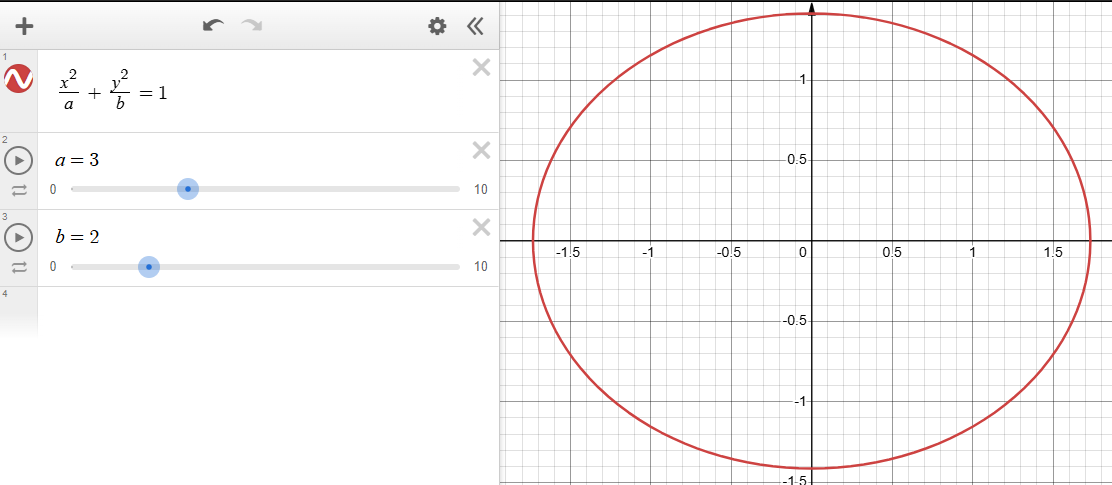
\includegraphics[width=0.6\textwidth]{images/ellipse.png}
\end{figure}

\textbf{Solution (c):}

Start with a circle of radius $r = 1$
    and suppose its area $A = \pi$.
We can subdivide this region into small squares with width $x$ and height $y$.
By Problem $3$ applying a $F_{a, b}$ to $x, y$ gives $ax, by$
    resulting in an area of $ab(xy)$.
Applying these dilations to the entire unit circle gives $ab\pi$.

\begin{tcolorbox}[title=Problem 7, breakable]
    Write up a discussion of how to give coordinates $(x, y, z)$ to 
    a point in $3-$space. In terms of these coordinates, what would the 
    effect of dilation by $r$?
\end{tcolorbox}

\textbf{Solution:}

Let $L_1, L_2, L_3$ be perpendicular lines intersecting at a point $O$.
Let $P$ be an arbitrary point in space.
Let the distances of the segments formed by dropping perpendiculars
    from $P$ to $L_1, L_2, L_3$ on one side be $(x, y, z)$.
On the opposite side, they are $(-x, -y, -z)$.

Let $V$ be the volume of a region in $3$-space. The effect of 
a dilation by $r$ would be to multiply the volume by $r^3$, giving $r^3 V$.

\begin{tcolorbox}[title=Problem 8, breakable]
    Generalize the discussion of this section to the $3$-dimensional
    case. Specifically:

    (a) Under dilation by $r$, how does the volume of a cube change?

    (b) How does the volume of a rectangle box with sides $a, b, c$ change?
        Draw a picture, say $r = \frac{1}{2}, r = 2, r = 3$, arbitrary $r$.

    (c) How would the volume of a $3-$dimensional solid change under 
        dilation by $r$?

    (d) The volume of the solid ball of radius $1$ in $3-$space is equal 
        to $\frac{4}{3} \pi$. What is the volume of the ball of radius 
        $r$ in $3-$space?
\end{tcolorbox}

\textbf{Solution (a):}

Under dilation $r$ the new volume $V' = r^3 V$ where $V$ is the volume 
    of the original cube.

\textbf{Solution (b):}

\begin{figure}[h]
    \centering
    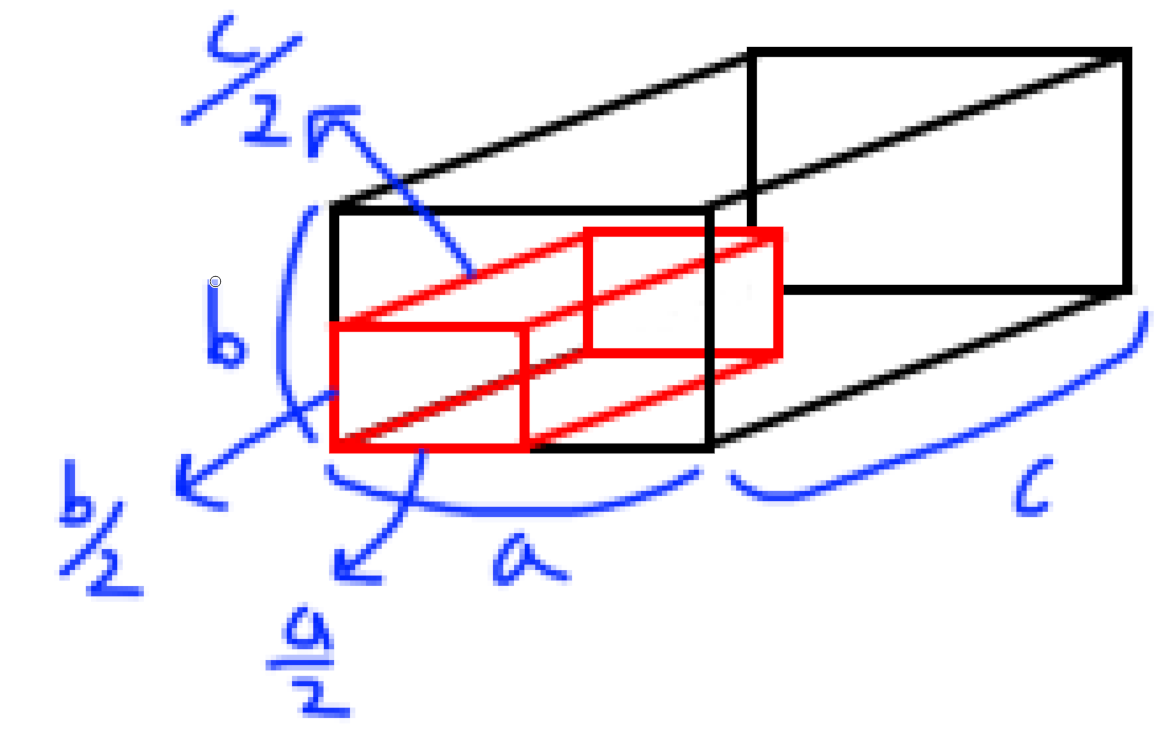
\includegraphics[width=0.6\textwidth]{images/half_rect.png}
\end{figure}

\begin{figure}[h]
    \centering
    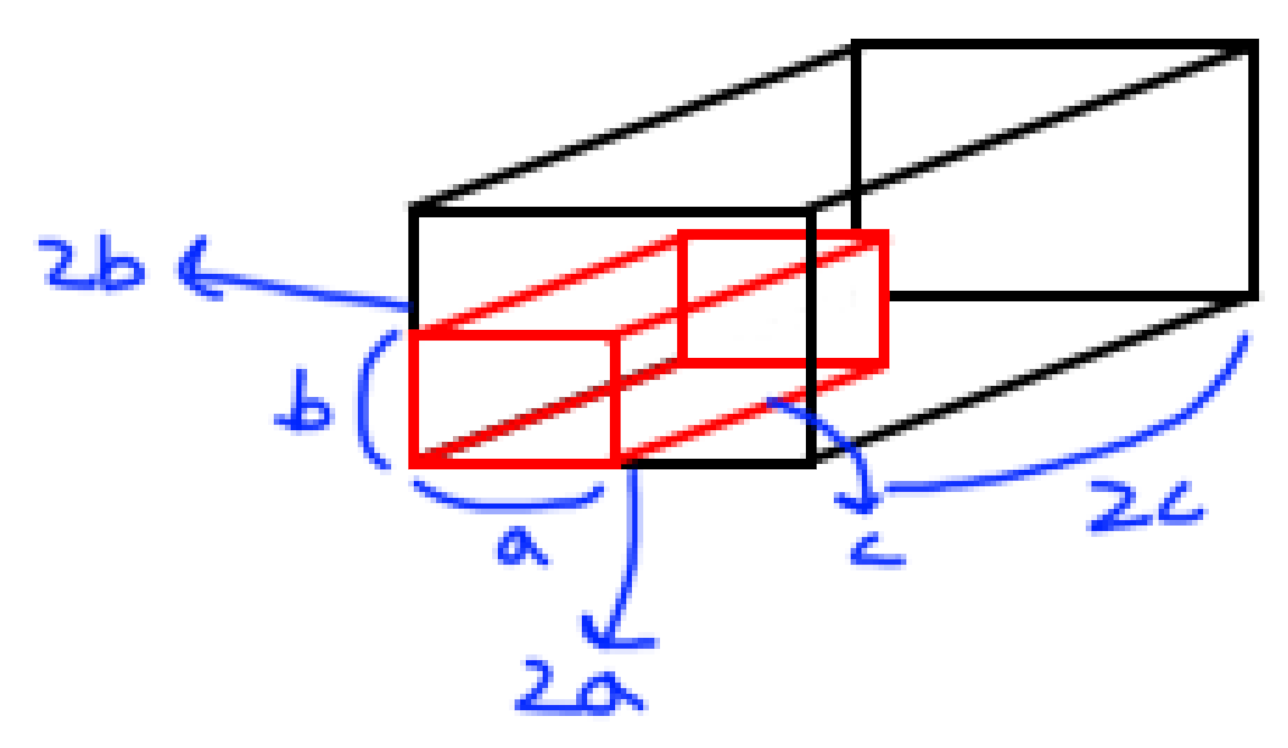
\includegraphics[width=0.6\textwidth]{images/2_rect.png}
\end{figure}

\begin{figure}[h]
    \centering
    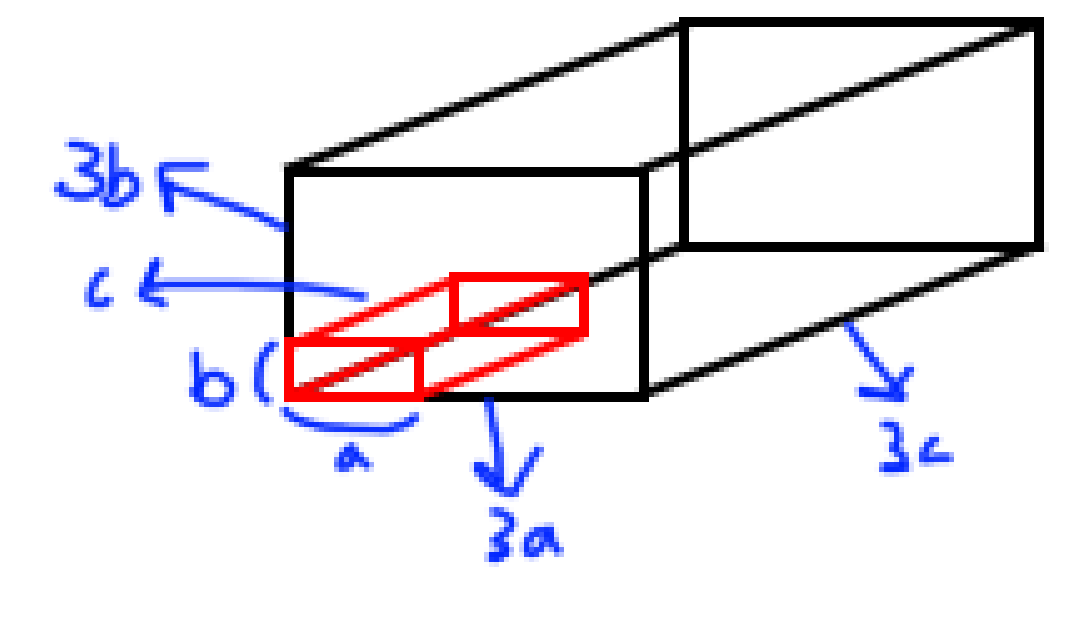
\includegraphics[width=0.6\textwidth]{images/3_rect.png}
\end{figure}

There are three cases for an arbitrary $r$ shown below
    depending on if $r < 1, r = 1, r > 1$.
If $r = 1$ the rectangle doesn't change that image isn't shown.
The first image shows if $r < 1$ and the second shows if $r > 1$.

\begin{figure}[h]
    \centering
    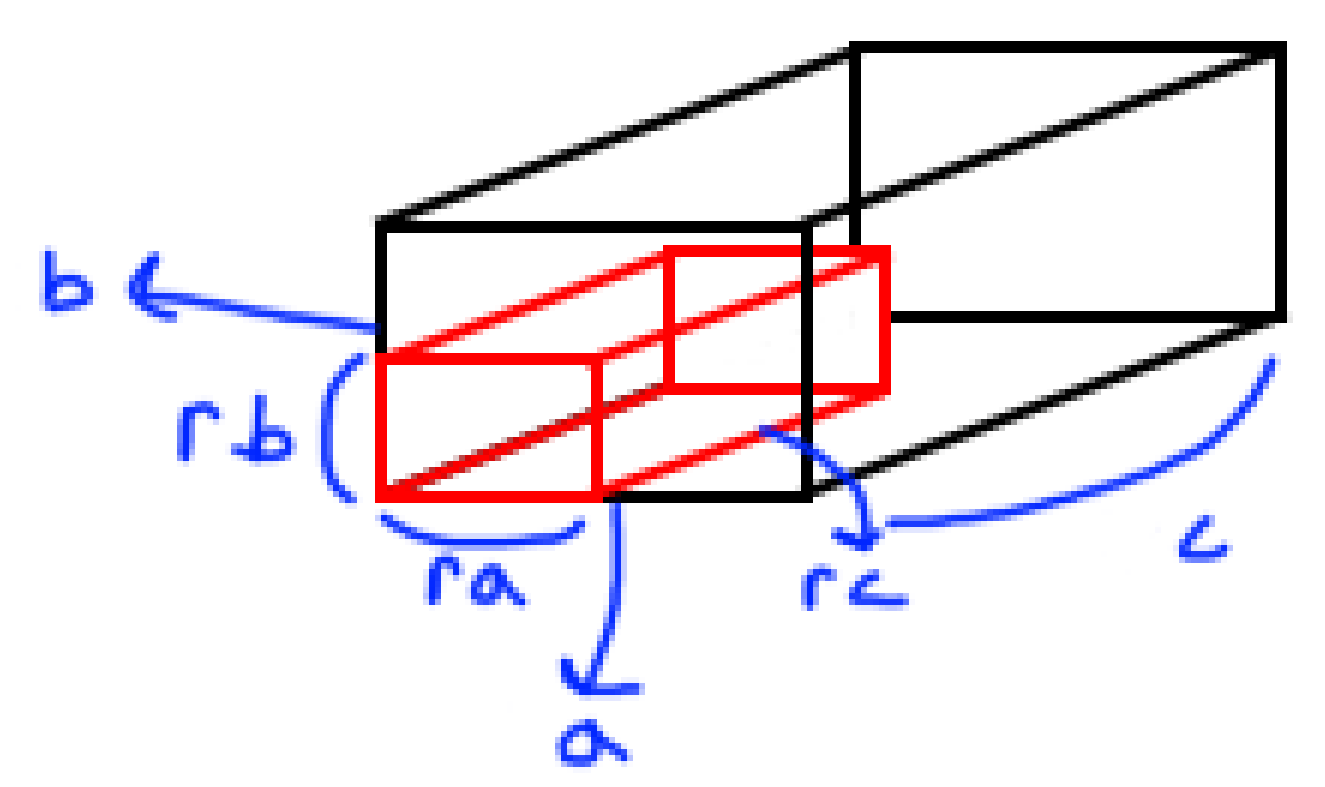
\includegraphics[width=0.6\textwidth]{images/arb1_rect.png}
\end{figure}

\begin{figure}[h]
    \centering
    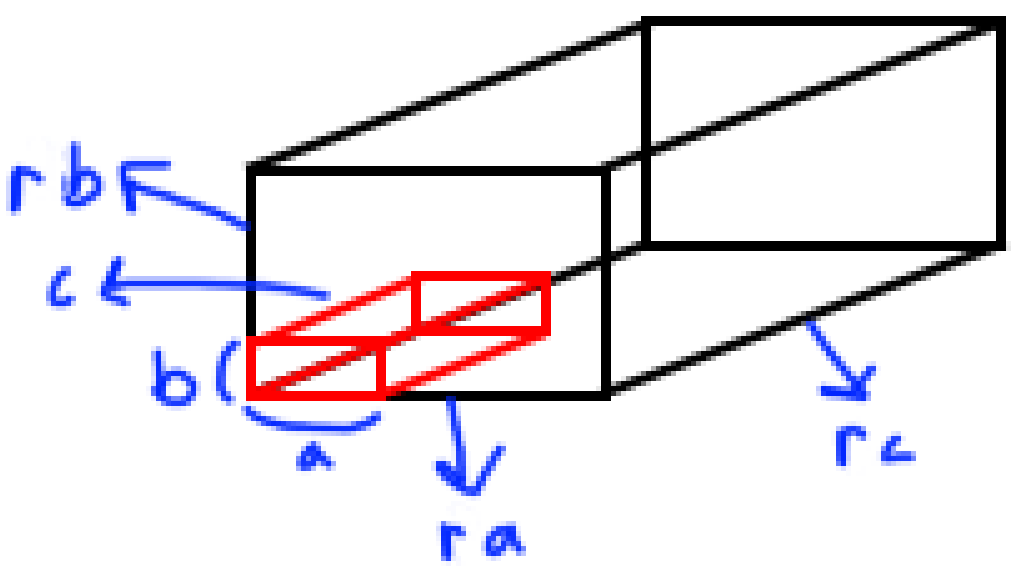
\includegraphics[width=0.6\textwidth]{images/arb2_rect.png}
\end{figure}

\textbf{Solution (c):}

Let $V$ be the volume of a solid. Under dilation $r$ the volume of the 
new solid is 
\[r^3 \cdot V\]

\textbf{Solution (d):}

\[V = r^3 \cdot \frac{4}{3}\pi\]

\begin{tcolorbox}[title=Problem 9, breakable]
    Write down the equation of a sphere of radius $r$ centered at the 
    origin in $3-$space.
\end{tcolorbox}

\textbf{Solution:}
\[a^2 + b^2 + c^2 = r^2\]

\begin{tcolorbox}[title=Problem 10, breakable]
    How would you define the volume of a rectangle solid whose sides 
    have lengths $a, b, c$.
\end{tcolorbox}

\begin{definition}
    Let the volume $V$ of a rectangle $R$ be defined as
    \[V = a \cdot b \cdot c\]
\end{definition}

\begin{tcolorbox}[title=Problem 11, breakable]
    Let $a, b, c$ be positive numbers. Let $\mathbb{R}^3$ be $3-$space,
    that is, the set of all triples of numbers $(x, y, z)$. Let 
    \[F_{a, b, c}: \mathbb{R^3} \rightarrow \mathbb{R}^3\]
    be the mapping
    \[(x, y, z) \rightarrow (ax, by, cz)\]
    Thus $F_{a, b, c}$ is a generalization to a $3-$space of our mixed 
    dilation $F_{a, b}$.

    (a) What is the image of a cube whose sides have length $1$ under $F_{a, b, c}$?
    
    (b) A rectangular box $S$ has sides of length $r, s, t$ respectively.
        What are the lengths of the sides of the image $F_{a, b}(S)$?
        What is the volume of $F_{a, b, c}(S)$?

    (c) Let $S$ be a solid in $3-$space, and let $V$ be its volume. 
        In terms of $V$, $a, b, c$ what is the volume of the image $S$
        under $F_{a, b, c}$?
\end{tcolorbox}

\textbf{Solution (a):}

The image of a cube whose sides have length $1$ under $F_{a, b, c}$
is a rectangular prism of side lengths $a, b, c$.

\textbf{Solution (b):}

The lengths of the sides of the image $F_{a, b}(S)$ is $ar, bs, t$.
The volume of $F_{a, b, c}(S)$ is $V = abc(rst)$.

\textbf{Solution (c):}

Let $V'$ be the volume of the image.
\[V' = abc V\]

\begin{tcolorbox}[title=Problem 12, breakable]
    What is the volume of the solid in $3-$space consisting of all points
    $(x, y, z)$ satisfying the inequality
    \[\left(\frac{x}{3}\right)^2 + \left(\frac{y}{2}\right)^2 + \left(\frac{z}{7}\right)^2 \le 1\]
\end{tcolorbox}

\textbf{Solution:}
\[V = 3 \cdot 2 \cdot 7 \cdot \frac{4}{3} \pi\]

\begin{tcolorbox}[title=Problem 14, breakable]
    Let $a, b, c$ be numbers $>0$. What is the volume of the solid 
    in $3-$space consisting of all points $(x, y, z)$ satisfying
    the inequality
    \[\left(\frac{x}{a}\right)^2 + \left(\frac{y}{b}\right)^2 + \left(\frac{z}{c}\right)^2 \le 1\]
\end{tcolorbox}

\textbf{Solution:}
\[V = a \cdot b \cdot c \cdot \frac{4}{3} \pi\]

\begin{tcolorbox}[title=Problem 15, breakable]
    What about $4-$space? $n-$space for arbitrary $n$?
\end{tcolorbox}

Let $V'$ be volume of $4-$D sphere.
The volume of the solid 
    in $4-$space consisting of all points $(x, y, z, d)$ satisfying
    the inequality
\[\left(\frac{x}{a}\right)^2 + \left(\frac{y}{b}\right)^2 
+ \left(\frac{z}{c}\right)^2 + \left(\frac{p}{d}\right)^2 \le 1\]
has volume
\[V = a \cdot b \cdot c \cdot d \cdot V'\]

Let $V'$ be volume of $n-$D sphere.
The volume of the solid 
    in $n-$space consisting of all points $(x_1, x_2, x_3, \ldots, x_n)$ satisfying
    the inequality
\[\left(\frac{y_1}{x_1}\right)^2 + \left(\frac{y_2}{x_2}\right)^2 
+ \left(\frac{y_3}{x_3}\right)^2 + \ldots +  \left(\frac{y_n}{x_n}\right)^2 \le 1\]
has volume
\[V = x_1 \cdot x_2 \cdot x_3 \cdot \ldots \cdot x_n \cdot V'\]
% Week 2: Focus on limit laws, one-sided limits, and indeterminate forms. Practice evaluating limits algebraically and with L'Hôpital's Rule.

\section{Continuity}
\subsection{Coordinate Systems}

\begin{tcolorbox}[title=Problem 3, breakable]
    Let $(x, y)$ be the coordinates of a point
    in the second quadrant.
    Is $x$ positive or negative?
    Is $y$ positive or negative?
\end{tcolorbox}

\textbf{Solution:}

The $x$ is negative.
The $y$ is positive.

\begin{tcolorbox}[title=Problem 4, breakable]
    Let $(x, y)$ be the coordinates of a point in the 
    third quadrant. Is $x$ positive or negative.
    Is $y$ positive or negative.
\end{tcolorbox}

The $x$ is negative.
The $y$ is negative.

\subsection{Distance Between Points}

\begin{tcolorbox}[title=Problem 11, breakable]
    Prove that if $d(P, Q) = 0$, then $P = Q$. Thus we have now 
    proved two of the basic properties of distance.
\end{tcolorbox}

\begin{proof}
    Suppose $P \ne Q$. Let $(x_1, x_2) = P$ and $(y_1, y_2) = Q$.
    Either $x_1 \ne y_1$ or $x_2 \ne y_2$.

    Suppose $x_1 \ne y_1$. It follows that $x_1 - y_1 \ne 0$
    and therefore, since $(x_2 - y_2)^2 \ge 0$, $\sqrt{(x_1 - y_1)^2 + (x_2 - y_2)^2} \ne 0$.
    Thus $d(P, Q) \ne 0$.

    Suppose $x_2 \ne y_2$. It follows similarly that $d(P, Q) \ne 0$.

    Therefore, if $d(P, Q) = 0$, then $P = Q$.
\end{proof}

\begin{tcolorbox}[title=Problem 12, breakable]
    Let $A = (a_1, a_2)$ and $B = (b_1, b_2)$.
    Let $r$ be a positive number.
    Write down the formula for $d(A, B)$.
    Define the \textbf{dilation} $r A$ be 
    \[r A = (r a_1, r a_2)\]
    For instance, if $A = (-3, 5)$ and $r = 7$,
    then $r A = (-21, 35)$. Prove in general that 
    \[d(r A, r B) = r \cdot d(A, B)\]
\end{tcolorbox}

\textbf{Solution:}

\[d(A, B) = \sqrt{(a_1 - b_1)^2 + (a_2 - b_2)^2}\]

\begin{proof}
    \begin{align*}
        d(rA, rB) &= \sqrt{(r a_1 - r b_1)^2 + (r a_2 - r b_2)^2} \\
                  &= \sqrt{(r^2 a_1^2 - r^2 a_1 b_1 - r^2 a_1 b_1 + r^2 b_1^2) + (r^2 a_2^2 - r^2 a_2 b_2 - r^2 a_2 b_2 + r^2 b_2^2)} \\
                  &= \sqrt{r^2 (a_1^2 - 2 a_1 b_1 + b_1^2 +  a_2^2 - 2 a_2 b_2 + b_2^2)} \\
                  &= r \sqrt{(a_1 - b_1)^2 + (a_2 - b_2)^2} \\
                  &= r d(A, B)
    \end{align*}
    Therefore, $d(rA, rB) = r d(A, B)$.
\end{proof}

\subsection{Equations of a Circle}

\begin{tcolorbox}[title=Problem 19, breakable]
    (a) Write down the equation for a sphere of radius $1$ centered
        at the origin in $3-$space, in terms of coordinates $(x, y, z)$.

    (b) Same question for a sphere of radius $3$.

    (c) Same question for a sphere of radius $r$.
\end{tcolorbox}

\textbf{Solution (a):}
\[x^2 + y^2 + z^2 = 1\]
\textbf{Solution (b):}
\[x^2 + y^2 + z^2 = 9\]
\textbf{Solution (c):}
\[x^2 + y^2 + z^2 = r^2\]

\subsection{Rational Points on a Circle}

\begin{tcolorbox}[title=Problem 2, breakable]
    Prove that if $s$, $t$ are real numbers such that $0 \le s < t$, then 
    \[\frac{1 - s^2}{1 + s^2} > \frac{1 - t^2}{1 + t^2}\]
    [Hint: Prove appropriate inequalities for the numerators and denominators,
    before taking the quotient.] This proves that different values for $t > 0$
    already give different values for $x$.
\end{tcolorbox}

\begin{proof}
    Suppose $s, t$ are real numbers such that $0 \le s < t$.

    Since $s < t$ it follows that $s^2 < t^2$ and $s^2 - t^2 < 0$.
    Then 
    \begin{align*}
        (1 - s^2) - (1 - t^2) 
            &= 1 - s^2 - 1 + t^2 \\
            &= -s^2 + t^2 \\
            &= -(s^2 - t^2)
    \end{align*}
    Since $s^2 - t^2 < 0$, it follows that $-(s^2 - t^2) > 0$.
    Thus $1 - s^2 > 1 - t^2$.

    Also
    \begin{align*}
        (1 + s^2) - (1 + t^2) 
            &= 1 + s^2 - 1 - t^2 \\
            &= s^2 - t^2 < 0
    \end{align*}
    Thus $1 + s^2 < 1 + t^2$.
    
    Since $1 - s^2 > 1 - t^2$ and $1 + s^2 < 1 + t^2$ 
        it follows that $(1 - s^2)(1 + t^2) > (1 - t^2)(1 + s^2)$.
    Therefore $\frac{1 - s^2}{1 + s^2} > \frac{1 - t^2}{1 + t^2}$
\end{proof}

\begin{tcolorbox}[title=Problem 4, breakable]
    When $t$ becomes very large positive, what happens to 
    \[\frac{1 - t^2}{1 + t^2}\]
    When $t$ becomes very large negative, what happens to 
    \[\frac{1 - t^2}{1 + t^2}\]
    Substitute large values of $t$, like $10,000$ or $-10,000$, to get 
    a feeling for what happens.
\end{tcolorbox}

\textbf{Solution:}

Let $t = 10000$ then
\[\frac{1 - t^2}{1 + t^2} = \frac{1 - (10000)^2}{1 + (10000)^2} = -0.9999998\]
As $t$ becomes very large positive $\frac{1 - t^2}{1 + t^2}$ approaches $-1$.

At $t = -10000$ it also approaches $-1$ since $t$ is squared it doesn't make a difference.

\begin{tcolorbox}[title=Problem 5, breakable]
    Analyze what happens to 
    \[\frac{2t}{1 + t^2}\]
    when $t \le 0$ and when $t$ becomes very large negative.
    Next analyze what happens when $t \ge 0$ and $t$ becomes 
    very large positive.
\end{tcolorbox}

Let $t = -10000$ then
\[\frac{2t}{1 + t^2} = \frac{2(-10000)}{1 + (-10000)^2} = −0.0002\]
As $t$ becomes very large negative $\frac{2t}{1 + t^2}$ approaches $0$.

Let $t = 10000$ then
\[\frac{2t}{1 + t^2} = \frac{2(10000)}{1 + (10000)^2} = 0.0002\]
As $t$ becomes very large positive $\frac{2t}{1 + t^2}$ approaches $0$.
% Week 3: Understand continuity and discontinuities. Connect with limits. Know Intermediate Value Theorem applications.

\section{The Derivative}
\subsection{Dilations and Reflections}

\begin{tcolorbox}[title=Problem 2, breakable]
    Let $A$ be a point, $A \ne 0$. If $b, c$ are numbers 
    such that $b A = c A$, prove that $b = c$.
\end{tcolorbox}

\begin{proof}
    Let $A = (a_1, a_2)$. Then $b A = (b a_1, b a_2)$
        and $c A = (c a_1, c a_2)$.
    Suppose $b A = c A$.
    Then $b a_1 = c a_1$ and $b a_2 = c a_2$.
    Since $A \ne 0$ either $a_1 \ne 0$ or $a_2 \ne 0$.
    Suppose $a_1 \ne 0$ then since $b a_1 = c a_1$
        dividing by $a_1$ shows $b = c$.
    Suppose $a_2 \ne 0$ then since $b a_2 = c a_2$
        dividing by $a_2$ shows $b = c$.

    Therefore $b = c$.
\end{proof}

\begin{tcolorbox}[title=Problem 3, breakable]
    Prove that reflection through $O$ preserves distances.
    In other words, prove that 
    \[d(A, B) = d(-A, -B)\]
\end{tcolorbox}

\begin{proof}
    Let $A = (a_1, a_2)$ and $B = (b_1, b_2)$. Then
    \[
    d(-A, -B) = \sqrt{((-a_1)-(-b_1))^2 + ((-a_2)-(-b_2))^2}
    = \sqrt{(a_1 - b_1)^2 + (a_2 - b_2)^2} = d(A, B).
    \]
\end{proof}

\begin{tcolorbox}[title=Problem 4, breakable]
    \textbf{The $3-$ dimensional case}

    (a) Define the multiplication (dilation) of a point $A = (a_1, a_2, a_3)$
        by a number $c$. Write out interpretations for this similar to those 
        we did in the plane. Draw pictures.

    (b) Define reflection $A$ through $O = (0, 0, 0)$.

    (c) State and prove the analogs of Theorems $1$ and $2$.
\end{tcolorbox}
\begin{figure}[h]
    \centering
    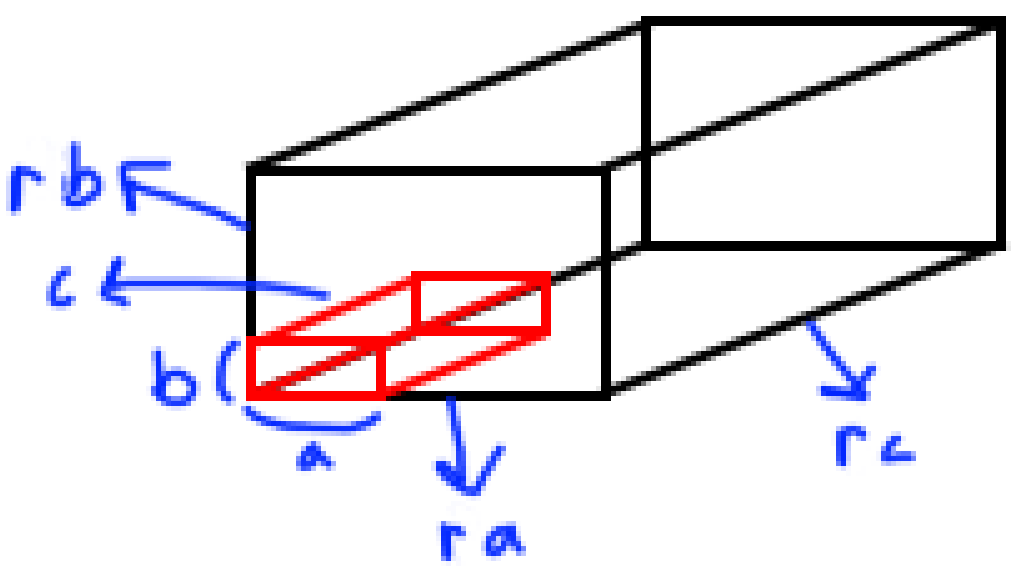
\includegraphics[width=0.6\textwidth]{images/arb2_rect.png}
\end{figure}
\begin{definition}
    Let $r$ be a real number.
    Let the dilation of a point $A = (a_1, a_2, a_3)$ by $r$ be defined as follows
    \[r A = (r a_1, r a_2, r a_3)\]
\end{definition}
\begin{definition}
    Let the reflection $R$ of $A$ through $O = (0, 0, 0)$
    dilation with $r = -1$.
\end{definition}
\begin{theorem}
    Let $r$ be a postiive number. If $A, B$ are points, then 
    \[d(A, B) = r \cdot d(A, B)\]
\end{theorem}
\begin{proof}
    Let $A = (a_1, a_2, a_3)$ and $B = (b_1, b_2, b_3)$.
    Then $r A = (r a_1, r a_2, r a_3)$ and $r B = (r b_1, r b_2, r b_3)$.
    Hence 
    \begin{align*}
        d(r A, r B)^2 
            &= (r b_1 - r a_1)^2 + (r b_2 - r a_2)^2 + (r b_3 - r a_3)^2 \\
            &= (r (b_1 - a_1))^2 + (r (b_2 - a_2))^2 + (r (b_3 - a_3))^2 \\
            &= r^2(b_1 - a_1)^2 + r^2(b_2 - a_2)^2 + r^2(b_3 - a_3)^2 \\
            &= r^2 \cdot d(A, B)^2
    \end{align*}
    Taking the square root proves our theorem.
\end{proof}
\begin{theorem}
    Let $c$ be a number. Then 
    \[d(c A, c B) = |c| \cdot d(A, B)\]
\end{theorem}
\begin{proof}
    Let $A = (a_1, a_2, a_3)$ and $B = (b_1, b_2, b_3)$.
    Then $c A = (c a_1, c a_2, c a_3)$ and $c B = (c b_1, c b_2, c b_3)$.
    Hence 
    \begin{align*}
        d(c A, c B)^2 
            &= (c b_1 - c a_1)^2 + (c b_2 - c a_2)^2 + (c b_3 - c a_3)^2 \\
            &= (c (b_1 - a_1))^2 + (c (b_2 - a_2))^2 + (c (b_3 - a_3))^2 \\
            &= c^2(b_1 - a_1)^2 + c^2(b_2 - a_2)^2 + c^2(b_3 - a_3)^2 \\
            &= c^2 \cdot d(A, B)^2
    \end{align*}
    Taking the square root proves our theorem since $\sqrt{c^2} = |c|$.
\end{proof}

\subsection{Addition, Subtraction, and Parallelogram Law}

\begin{tcolorbox}[title=Problem 11, breakable]
    Let $T_A$ be a translation by $A$. Prove that it is an isometry,
    in other words, that for any pair of points $P, Q$ we have 
    \[d(P, Q) = d(T_A(P), T_A(Q))\]
\end{tcolorbox}

\begin{proof}
    Let $P = (p_1, p_2), Q = (q_1, q_2), A = (a_1, a_2)$.
    Now $d(P, Q) = \sqrt{(p_1 - q_1)^2 + (p_2 - q_2)^2}$.
    Then $d(T_A(P), T_A(Q)) 
        = \sqrt{((p_1 + a_1)^2 - (q_1 + a_1)^2) + ((p_2 + a_2) - (q_2 + a_2))^2}
        = \sqrt{(p_1^2 + 2 p_1 a_1 + a_1^2 - q_1^2 - 2 q_1 a_1 - a_1^2) + ()} $.
\end{proof}

\begin{tcolorbox}[title=Problem 12, breakable]
    Let $D(r, A)$ denote the disc of radius $r$ centered at $A$.
    Show that $D(r, A)$ is the translation of $A$ of the disc $D(r, O)$
    of radius $r$ centered at $O$.
\end{tcolorbox}

\begin{tcolorbox}[title=Problem 13, breakable]
    Let $S(r, P)$ denote the circle of radius $r$ centered at $P$.

    (a) Show that the reflection of this circle through $O$ is a again a circle.
        What is the center of the reflected circle.

    (b) Show that the reflection of the disc $D(r, P)$ through $O$ is a disc.
        What is the center of this reflected disc?
\end{tcolorbox}

\begin{tcolorbox}[title=Problem 14, breakable]
    Let $P, Q$ be points. Write $P = Q + A$, where $A = P - Q$. Define 
    the \textbf{reflection of $P$ through $Q$} to be the point $Q - A$.
    If $R_Q$ denotes reflection through $Q$, tehn we have $R_Q(P) = 2 Q - P$.
    (Why?) Draw the picture, showing $P, Q, A$ and $Q - A$ to convince yourself
    that this definition corresponds to our geometric intuition.
\end{tcolorbox}

\begin{tcolorbox}[title=Problem 15, breakable]
    (a) Prove that reflection through a point $Q$ can be expressed in terms 
        of reflection through $O$, followed by a translation.

    (b) Let $T_A$ be translation by $A$, and $R_0$ reflection with respect 
        to teh origin. PRove that the composite $T_A \circ R_0$ is equal 
        to $R_Q$ for some point $Q$. Which one?
\end{tcolorbox}

\begin{tcolorbox}[title=Problem 16, breakable]
    (a) Let $r$ be a positive number.
        Give an analytic definition of \textbf{dilation by $r$ with respect to a point $Q$},
        and denote this dilation by $F_{r, Q}$. To give this definition, look at 
        Excersize $14$. You may also want to look at the discussion about line segments
        in $4$. If $P$ is a point, draw the picture with $O, P, Q, P - Q$, and $F_{r, Q}(P)$.

    (b) From your definition, it should be clear that $F_{r, Q}$ can be obtained as a composite 
        of dilation with respect to $O$, and a translation. Translation by what point?
\end{tcolorbox}

\begin{tcolorbox}[title=Problem 17, breakable]
    Let $S(r, A)$ be the circle of radius $r$ and center $A$.
    Show that the reflection of this circle through a point $Q$ is a circle.
    What is the center of this reflected circle?
    What is its radius?
    Draw a picture.
\end{tcolorbox}

\begin{tcolorbox}[title=Problem 18, breakable]
    The inverse of the translation $T_A$ is also a translation.
    By what? Prove your assertion.
\end{tcolorbox}

\begin{tcolorbox}[title=Problem 19, breakable]
    Let $F_r$ be dilation by a postive number $r$,
    with respect to $O$, and let $T_A$ be a translation by $A$.

    (a) Show that $F_r^{-1}$ is also a dilation. By what number?

    (c) Show that $F_R \circ T_A \circ F_r^{-1}$ is a translation.
\end{tcolorbox}

\begin{tcolorbox}[title=Problem 20, breakable]
    Show that the composite of two translations is a translation.
    $T_A \circ T_B = T_C$, how would you express $C$ in terms 
    of $A$ and $B$?
\end{tcolorbox}

\begin{tcolorbox}[title=Problem 21, breakable]
    Let $R$ be a reflection through the origin.

    (a) Show that $R^{-1}$ exists.

    (b) Show that $R \circ T_A \circ R^{-1}$ is a translation. By what?
\end{tcolorbox}

\begin{tcolorbox}[title=Problem 22, breakable]
\end{tcolorbox}

\begin{tcolorbox}[title=Problem 23, breakable]
\end{tcolorbox}

\begin{tcolorbox}[title=Problem 24, breakable]
\end{tcolorbox}

\begin{tcolorbox}[title=Problem 25, breakable]
\end{tcolorbox}

\begin{tcolorbox}[title=Problem 26, breakable]
\end{tcolorbox}

\begin{tcolorbox}[title=Problem 29, breakable]
\end{tcolorbox}

\begin{tcolorbox}[title=Problem 30, breakable]
\end{tcolorbox}

\begin{tcolorbox}[title=Problem 31, breakable]
\end{tcolorbox}

\begin{tcolorbox}[title=Problem 32, breakable]
\end{tcolorbox}
% Week 4: Focus on definition of derivative, basic rules, and interpreting derivatives as rates of change and slopes.

\section{Rules for Differentiating Functions}
\input{sections/chapter10.tex}
% Week 5: Product, quotient, chain rule. Drill multiple examples to build speed.

\section{Implicit Differentiation}
\input{sections/chapter11.tex}
% Week 6: Learn to differentiate equations not solved for y. Practice solving for dy/dx in complex examples.

\section{Tangent and Normal Lines}
\input{sections/chapter12.tex}
% Week 7: Connect derivatives to geometric interpretation. Practice tangent lines and normals.

\section{Increasing/Decreasing and Mean Value Theorem}
\input{sections/chapter13.tex}
% Week 8: Focus on identifying intervals of increase/decrease, concavity, and applying MVT.

\section{Maximum and Minimum Values}
\input{sections/chapter14.tex}
% Week 9: Practice finding local and global extrema. Connect with derivative tests.

\section{Curve Sketching, Concavity, Symmetry}
\input{sections/chapter15.tex}
% Week 10: Combine derivative info to sketch curves. Focus on interpreting concavity and inflection points.

\section{Differentiation of Trigonometric Functions}
\input{sections/chapter17.tex}
% Week 11: Review derivatives of sin, cos, tan, etc. Practice chain rule with trig functions.

\section{Inverse Trigonometric Functions}
\input{sections/chapter18.tex}
% Week 12: Learn derivatives of arcsin, arccos, arctan, etc. Connect to implicit differentiation.

\section{Related Rates}
\input{sections/chapter20.tex}
% Week 13: Focus on translating word problems into derivative equations. Practice multiple real-world scenarios.

\section{Differentials and Newton's Method}
\input{sections/chapter21.tex}
% Week 14: Understand differentials, linear approximations, and Newton-Raphson root-finding.

\section{Antiderivatives}
\input{sections/chapter22.tex}
% Week 15: Review basic antiderivatives, power rule, and substitution.

\section{Definite Integral and Area Under a Curve}
\input{sections/chapter23.tex}
% Week 16: Connect Riemann sums to definite integrals. Practice area computations.

\section{Fundamental Theorem of Calculus}
\input{sections/chapter24.tex}
% Week 17: Understand both parts of the theorem and applications to evaluating integrals.

\section{Applications: Area and Arc Length}
\input{sections/chapter29.tex}
% Week 18: Solve area between curves and arc length problems.

\section{Applications: Volume}
\input{sections/chapter30.tex}
% Week 19: Focus on disk, washer, and shell methods. Practice multiple setup problems.

\section{Techniques of Integration I: Integration by Parts}
\input{sections/chapter31.tex}
% Week 20: Practice by parts on polynomial × trig/exponential functions.

\section{Techniques of Integration II: Trig Integrands / Trig Substitutions}
\input{sections/chapter32.tex}
% Week 21: Focus on trig integrals and substitutions. Recognize patterns quickly.

\section{Techniques of Integration III: Partial Fractions}
\input{sections/chapter33.tex}
% Week 22: Practice decomposing rational functions and integrating. Very common in Calc 3 review.

\section{Improper Integrals}
\input{sections/chapter35.tex}
% Week 23: Understand convergence/divergence and setup of improper integrals.

\section{Parametric Representation of Curves}
\input{sections/chapter37.tex}
% Week 24: Review derivatives of parametric equations and tangent lines.

\section{Plane Vectors}
\input{sections/chapter39.tex}
% Week 25: Intro to vectors in 2D. Useful for moving into 3D vectors in Calc 3.

\section{Polar Coordinates}
\input{sections/chapter41.tex}
% Week 26: Practice plotting, derivatives, and areas in polar coordinates.

\section{Sequences}
\input{sections/chapter42.tex}
% Week 27: Understand limits of sequences and convergence intuition.

\section{Series}
\input{sections/chapter43.tex}
% Week 28: Practice convergence tests (integral, comparison, ratio, alternating). Do multiple examples.

\section{Power Series}
\input{sections/chapter46.tex}
% Week 29: Focus on representing functions as series and finding interval of convergence.

\section{Taylor and Maclaurin Series}
\input{sections/chapter47.tex}
% Week 30: Practice expansions of common functions (e^x, sin x, cos x, ln(1+x)). Connect derivatives to series coefficients.

\end{document}
